\chapter{Results}
\label{cha:Results}


\section{Eval for question 1}

The trained policy was evaluated on tracks of all difficulty settings with the standard light setting using the Basic Evaluation algorithm \ref{sec:eval_model_track} with 100 episodes per setting. The success rates for the different difficulty settings are shown in figure \ref{fig:result_success_rates_standard}. Example videos of the agent's behaviour during evaluation can be found in the appendix \ref{cha:example_videos}.

\subsection{Experiment Results}

\begin{figure}
    \centering
    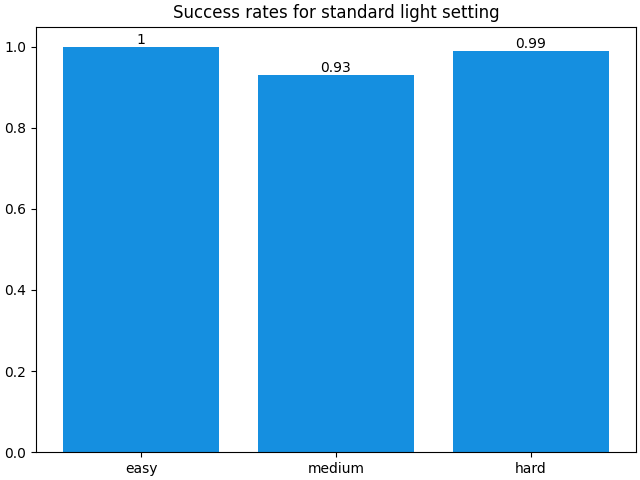
\includegraphics[width=0.45\textwidth]{Bilder/notebook_images/success_trainedHardStandardDistanceRewardEval_standard_success_rates_barplot.png}
    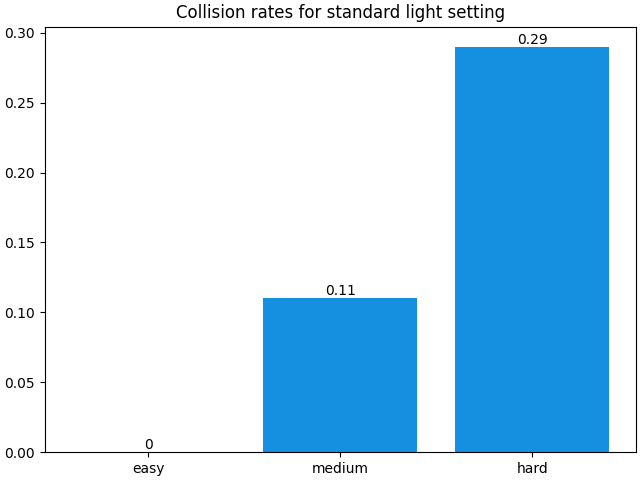
\includegraphics[width=0.45\textwidth]{Bilder/notebook_images/success_trainedHardStandardDistanceRewardEval_standard_collision_rates_barplot.png}
    \caption{Success and collision rates for standard light setting.}
    \label{fig:result_success_rates_standard}
\end{figure}


The policy completed the easy, medium and hard tracks with a succes\_rate of 100\%, 93\% and 97\%. The collision\_rates were 0\%, 11\% and  29\%. The collision rates increase for the higher difficulty tracks.

\subsection{Discussion}

The trained policy is able to complete all difficulty levels very reliably.
Especially for higher difficulty settings the agent does not avoid collisions completely. However the data shows that many of the collisions are minor and the agent is able to recover from them and complete the parcour.

The policy was trained on the difficult setting only. The policy did not see easy and medium difficulty parcours before the evaluation. The policy is able to generalize to tracks of lower difficulty.

\section{Eval for question 2}

The most succesfull model was used to evaluate the agent's performance under different light settings. The agent was evaluated on the standard, dark and bright light settings. Each combination of difficulty and light setting was evaluated with the Basic Evaluation Algorithm for 100 episodes. The success rates for the different light settings are shown in figure \ref{fig:result_success_rates_lightSettings}.


\subsection{Experiment Results}

\begin{figure}
    \centering
    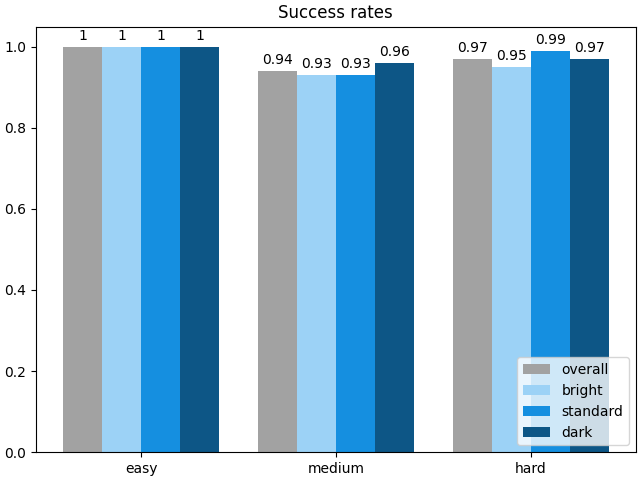
\includegraphics[width=0.45\textwidth]{Bilder/notebook_images/success_trainedHardStandardDistanceRewardEval_all_success_rates_barplot.png}
    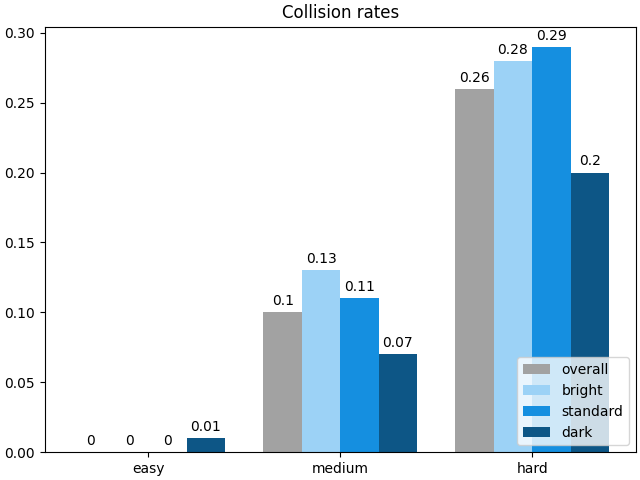
\includegraphics[width=0.45\textwidth]{Bilder/notebook_images/success_trainedHardStandardDistanceRewardEval_all_collision_rates_barplot.png}
    \caption{Success and collision rate comparisons for light settings.}
    \label{fig:result_success_rates_lightSettings}
\end{figure}

The success rates for all light and difficulty settings are very high. The evaluations for the bright and dark light settings show slight differences in performance compared to the standard light setting for medium and hard tracks. The light setting had no influence on the success\_rate for the easy tracks. The agent completed the easy tracks for all light settings with a success rate of 100\%.
Most notably the success rate for medium tracks even increased by 3\% percent for the dark setting. 

The collision rates changed much more significantly for the bright and dark setting compared to the standard setting. Some collision rates are higher for the bright and dark setting, some are lower. Overall the collision rates of difficulty levels did not change significantly compared to the standard light condition. The overall collision rate for the medium setting was 10\% compared to 11\% for the standard setting. The overall collision rate for the hard setting was 26\% compared to 29\% for the standard setting.
For the hard tracks, the collision rate for the dark setting is only 20\%, while the collision rate for the standard setting is 29\%. 

Across all light and difficulty settings the overall success rate is 97\% and the overall collision rate is only 12\%.

\subsection{Discussion}

The policy was able to complete the parcours very reliably under the different light settings. The light setting only had a small impact on the success rate.
The different light settings also did not lead to an overall increase in collisions.

The evaluated policy was trained on the standard light setting only. The policy did not see samples from the dark and bright light settings during training. The policy is still able to generalize to the bright and dark light settings.
This suggests that the histogram equalization proprocessing step plays an important role for this policy's behaviour.


\section{Eval for Question 3 - Replays}

The most successful model was used to record replays of the agent's behaviour. This most successful model used a $fixedTimestepLength$ of $0.3$ seconds. This means the hardware has to able to make a decision every $0.3$ seconds to be considered fast enough.

Five episodes were recorded for each difficulty and light setting combination. As expected from the previous evaluations of the policy, the replay episodes had a very high success\_rate of 97\%. The recorded episodes were then replayed on the Nvidia Jetbot. The time it took to replay the episodes was measured \ref{fig:result_replay_times}. The policy outputs from the replay were compared to the policy outputs from the recordings \ref{fig:result_replay_outputs}.


\begin{figure}
    \centering
    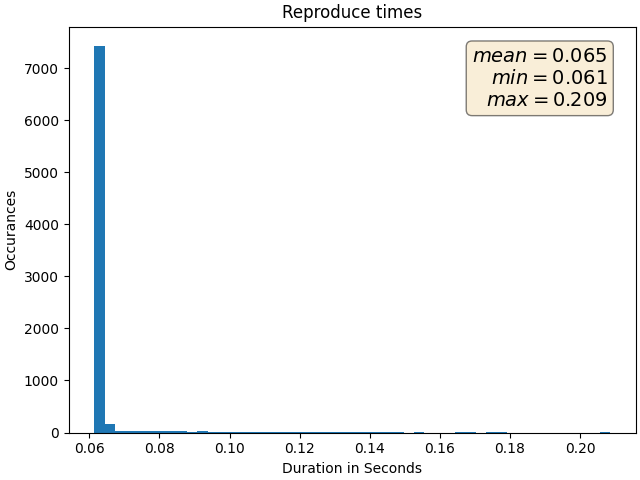
\includegraphics[width=0.8\textwidth]{Bilder/notebook_images/replay_times.png}
    \caption{Replay times on jetbot hardware}
    \label{fig:result_replay_times}
\end{figure} % a chart showing the replay times (max, min, mean)


\begin{figure}
    \centering
    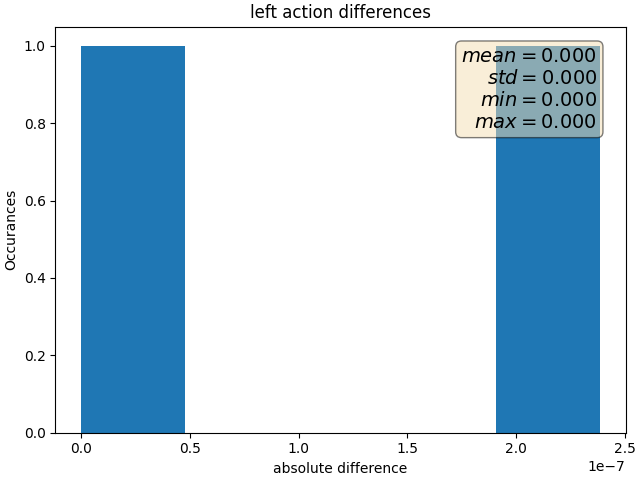
\includegraphics[width=0.45\textwidth]{Bilder/notebook_images/replay_outputs_action_left.png}
    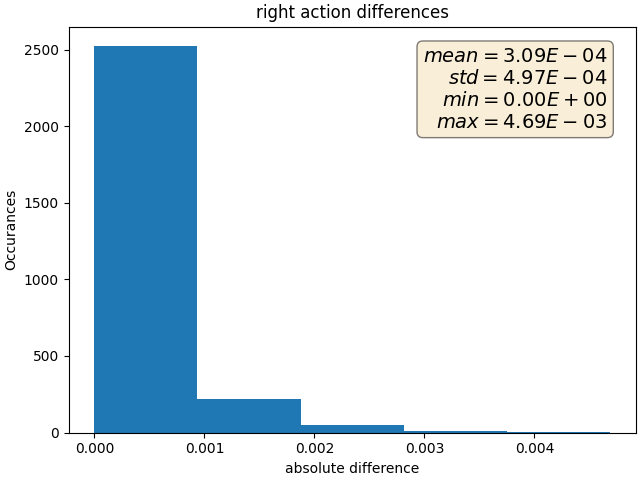
\includegraphics[width=0.45\textwidth]{Bilder/notebook_images/replay_outputs_action_right.png}
    \caption{Differences in policy outputs between recordings and replays on jetbot hardware}
    \label{fig:result_replay_outputs}
\end{figure} % a chart showing the replay times (max, min, mean) TODO change these outputs to use scientific notation


\subsection{Experiment Results}

\paragraph{Replay times}

The replay times for the recordings on jetbot hardware are shown in figure \ref{fig:result_replay_times}. The maximum duration was $0.208$ seconds. The mean is much lower at $0.065$ seconds. The plot shows that the maximum duration was an extreme outlier.
Given the $fixedTimestepLength$ of $0.3$ seconds and the maximum duration of $0.208$ seconds, the hardware is fast enough to replay the episodes. This leaves at least $0.091$ seconds for the agent to recieve an image from the camera and send the new instruction to the motors.


\paragraph{Policy Outputs}

The policy outputs from the recordings and the replays on jetbot hardware are nearly identical. The differences are shown in figure \ref{fig:result_replay_outputs}. The outputs were reproduced very closely. The maximum difference was $4.76e-07$.  This is difference is negligeable compared to the range of policy outputs $[-1,1]$.


\subsection{Discussion}

The jetbot hardware is capable enough to compute the policy in real time. The differences of the policy outputs between the recordings and the replays are very small, the policy outputs were reproduced very closely. This suggests the differences in hardware and software do not impact the policy significantly.


\section{Other experiments}

\subsection{Fresh obs improves}

fresh observation is slightly better than non-fresh observations
--> we can rerun the experiments for question 1 and 2 with fresh observations

\subsection{Test identical start conditions}


\subsection{Test deterministic improves}

non-deterministic results in better performance for this specific task


\subsection{Jetbot generalization}

...

